\chapter{Appendix}
    \section{Dagger}
        \label{appendix:dagger}
        Dagger is dependency injection framework. It is based on the 
        Java Specification Request (JSR) 330. 
        It uses code generation and is based 
        on annotations. The generated code is very relatively easy to read 
        and debug. It is the most popular dependency injection framework
        for android also used for java projects only.


    \begin{figure}[htbp!]
        \centering 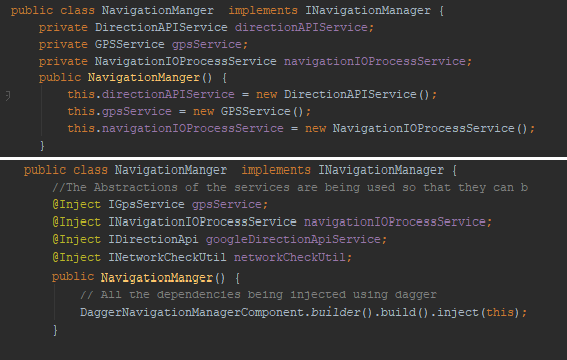
\includegraphics{grafiken/di_compare.png}
        \caption{Comparision of code with(bottom) and without Dependency injection(top)}
        \label{fig:DIComparision}
    \end{figure}